% !TEX root = main.tex
\chapter{Evaluation in a Dialog System}
\label{cha:integration}
This chapter discuss the details of interfacing a decoder from a dialog system.
Namely, Section~\ref{sec:integration} presents how the Python wrapper \term{PyOnlineLatgenRecogniser} was integrated 
into~\ac{SDS} Alex.
Section~\ref{sec:eval} evaluates the decoder in Alex dialogue system on Czech \ac{PTI} domain. 


\section{Integration of \term{OnlineLatgenRecogniser} into \ac{SDS}}
\label{sec:}
First the architecture of Alex \ac{SDS} is described in~Section~\ref{sec:arch}
and later we present the 

% section  (end)
\subsection{Dialog system architecture} 
\label{sec:arch}
The Alex dialog system is developed in Python language and consist of~six major components. 
\begin{enumerate}
    \item Voice Activity Detection (VAD)
    \item Automatic Speech Recognition (ASR) 
    \item Spoken Language Understanding (SLU)
    \item Dialog Manager (DM)
    \item Natural Language Generation (NLG)
    \item Text To Speech (TTS)
\end{enumerate}
The~Alex dialog system has a~speech to speech user interface. The~system interacts with the user in {\it turns}. During a~single turn the dialog system waits for a~user spoken input, process the speech and generates the reply.
The~data~flow during single turn is depicted in~Figure~\ref{fig:dialog_system}.

The integration task consist of:
\begin{itemize}
    \item Building a~Python interface for a~C++ Kaldi decoder.
    \item Define the input and output interface for the Kaldi decoder - wrapped by Automatic Speech Recognition (ASR) unit in Alex.
\end{itemize}
 The ASR unit takes output of~the VAD component and provides input for the SLU unit. 
 %The input and output interfaces are chosen according the real time needs of~the VAD unit and the SLU unit.

\begin{figure}
    \begin{center}
    % Generated with LaTeXDraw 2.0.5
% Wed Apr 09 16:50:40 CEST 2014
% \usepackage[usenames,dvipsnames]{pstricks}
% \usepackage{epsfig}
% \usepackage{pst-grad} % For gradients
% \usepackage{pst-plot} % For axes
\scalebox{1} % Change this value to rescale the drawing.
{
\begin{pspicture}(0,-3.66)(14.64,3.66)
\definecolor{color685}{rgb}{0.11764705882352941,0.14901960784313725,0.8901960784313725}
\definecolor{color523}{rgb}{0.027450980392156862,0.25882352941176473,0.8431372549019608}
\definecolor{color34}{rgb}{0.7843137254901961,0.0784313725490196,0.23529411764705882}
\psellipse[linewidth=0.04,dimen=outer](5.55,1.51)(0.83,0.69)
\usefont{T1}{ptm}{m}{n}
\rput(5.5046873,1.425){VAD}
\psellipse[linewidth=0.04,dimen=outer](8.97,2.61)(0.83,0.69)
\usefont{T1}{ptm}{m}{n}
\rput(8.942186,2.525){ASR}
\psellipse[linewidth=0.04,dimen=outer](12.51,1.15)(0.83,0.69)
\usefont{T1}{ptm}{m}{n}
\rput(12.455312,1.065){SLU}
\psellipse[linewidth=0.04,dimen=outer](12.61,-1.51)(0.83,0.69)
\usefont{T1}{ptm}{m}{n}
\rput(12.567813,-1.595){DM}
\psellipse[linewidth=0.04,dimen=outer](5.49,-1.27)(0.83,0.69)
\usefont{T1}{ptm}{m}{n}
\rput(9.001249,-2.315){NLG}
\psellipse[linewidth=0.04,dimen=outer](9.03,0.0)(5.61,3.66)
\usefont{T1}{ptm}{m}{n}
\rput(5.4315624,-1.355){TTS}
\psellipse[linewidth=0.04,dimen=outer](9.03,-2.23)(0.83,0.69)
\usefont{T1}{ptm}{m}{n}
\rput(9.0,0.24){\Huge Dialogue System}
\psline[linewidth=0.04cm,arrowsize=0.05291667cm 2.0,arrowlength=1.4,arrowinset=0.4]{->}(9.76,2.38)(11.9,1.6)
\psline[linewidth=0.04cm,arrowsize=0.05291667cm 2.0,arrowlength=1.4,arrowinset=0.4]{->}(6.36,1.76)(8.18,2.42)
\psline[linewidth=0.04cm,arrowsize=0.05291667cm 2.0,arrowlength=1.4,arrowinset=0.4]{->}(12.54,0.46)(12.56,-0.86)
\psline[linewidth=0.04cm,arrowsize=0.05291667cm 2.0,arrowlength=1.4,arrowinset=0.4]{->}(11.84,-1.74)(9.9,-2.32)
\psline[linewidth=0.04cm,arrowsize=0.05291667cm 2.0,arrowlength=1.4,arrowinset=0.4]{->}(8.14,-2.18)(6.3,-1.52)
\pscircle[linewidth=0.04,dimen=outer](0.98404694,2.1548762){0.6451238}
\psline[linewidth=0.04cm](1.0,1.0)(0.92,-0.16)
\psline[linewidth=0.04cm](0.98193634,1.0577894)(0.0,1.84)
\psline[linewidth=0.04cm](0.98193634,1.0432783)(2.0694895,2.1461184)
\psline[linewidth=0.04cm](0.9072397,-0.23489322)(1.46,-1.72)
\psline[linewidth=0.1cm,linecolor=color523,linestyle=dashed,dash=0.16cm 0.16cm,arrowsize=0.05291667cm 2.0,arrowlength=1.4,arrowinset=0.4]{->}(2.28,1.86)(4.46,1.5)
\psline[linewidth=0.1cm,linecolor=color523,linestyle=dashed,dash=0.16cm 0.16cm,arrowsize=0.05291667cm 2.0,arrowlength=1.4,arrowinset=0.4]{<-}(2.32,-0.52)(4.36,-0.88)
\usefont{T1}{ptm}{m}{n}
\rput(3.0603125,-1.055){\Large \color{color685}Speech}
\usefont{T1}{ptm}{m}{n}
\rput(3.0803125,1.345){\Large \color{color685}Speech}
\usefont{T1}{ptm}{m}{n}
\rput(6.8231244,2.605){\color{color34}Speech}
\usefont{T1}{ptm}{m}{n}
\rput(11.20875,2.605){\color{color34}Text/Lattice}
\usefont{T1}{ptm}{m}{n}
\rput(12.445,-0.435){\color{color34}Semantic meaning}
\usefont{T1}{ptm}{m}{n}
\rput(11.265624,-2.255){\color{color34}Action}
\usefont{T1}{ptm}{m}{n}
\rput(6.899688,-2.175){\color{color34}Text}
\psline[linewidth=0.04cm](0.8872397,-0.23489322)(0.1,-1.62)
\psline[linewidth=0.04cm](0.36193633,2.0032785)(1.72,2.76)
\psdots[dotsize=0.12](1.34,2.28)
\rput{48.07518}(1.8088533,-0.49558815){\psarc[linewidth=0.04](1.46,1.78){0.12}{0.0}{180.0}}
\psline[linewidth=0.04cm](1.0368464,1.4389827)(1.0031536,1.1610173)
\end{pspicture} 
}

    \caption{Single turn in Alex dialog system}
    \label{fig:dialog_system} 
    \end{center}
\end{figure}

In our dialog system we experiment with different outputs of~a~speech decoder in Spoken Language Understanding unit. 
The decoder for our system should be able to generate {\it n-best lists}, {\it lattices} and {\it confusion networks} output.
% Ideally, the decoder for our system would be able to generate {\it n-best lists}, {\it lattices} and {\it confusion networks}.

%   d) output of~the decoder will be standard lattices 
%     (both phone and word)
%   e) compute posterior lattices (both phone and word),
%   f) provide confusion networks for these lattices
%   g) measure teh quality of~the lattices, depth, oracle error rate    

% section integrate_kaldi_decoder_into_vystadial_framework (end)


% \subsection{Development of~a~real time decoder}
% \label{sub:kaldi_rt_decoder}
% In the our dialog system we need above all a~real time decoder for the Kaldi toolkit. At first, we will identify what prevents the current Kaldi decoders from being used as real time decoders. 
% 
% Namely, we will explore problems with latency and suggest potential speed improvements e.g.\ approximations, use of~\ac{GPU}, and so on. Based on the experiments we will suggest the optimal setting for the real time use of~Kaldi decoder.
% 
% % section development_of_real_time_asr_decoder_for_the_kaldi_toolkit (end)

We will also compare and contrast possibilities of~different output formats for each of~tested decoders. The~memory consumption and the~stability of~decoders will be also observed. 


\subsection{\term{PyOnlineLatgenRecogniser} as Alex ASR component}
\label{sub:asr_component}


\todo{Unused part from sigdial article, problem forward vs backward}





\section{Evaluation on Alex data}
\label{sec:eval}

\begin{figure*}[t]
    \begin{center}
    \includegraphics[scale=0.5]{beam_vs_rtfwer.pdf.ps}
    \includegraphics[scale=0.5]{latbeam_vs_latwer.pdf.ps}
    \caption{The~left graph (a) shows that WER decreases with increasing \term{beam} and the~average RTF linearly grows with the~beam.
    Setting the~maximum number of active states to 2000 stops the~growth of the~95th RTF percentile at 0.6, indicating that even in the~worst case, we can guarantee an~RTF around 0.6.
    The~right graph (b) shows how latency grows in response to increasing \term{lattice-beam}.}
    \label{fig:wer} 
    \end{center}
\end{figure*}

\subsection{Acoustic and language model training}
\label{sec:train}

The~\term{OnlineLatgenRecogniser} is evaluated on a~corpus of audio data from the~Public Transport Information (PTI) domain.
In PTI, users can interact in Czech language with a~telephone-based dialogue system to find public transport connections \cite{ptics2014url}.
The~PTI corpus consist of approximately 12k user utterances with a length varying between 0.4 s and 18 s with median around 3 s.
% The~data were divided into training, development, and test data where the~corresponding data sizes were 9496, 1188, 1188 respectively.
The~data were divided into training and test data, consisting of 10999 and 1223 utterances respectively.
For evaluation, a~domain specific class-based language model with a vocabulary size of approximately 52k  and 559k n-grams was estimated from the~training data.
Named entities e.g., cities or bus stops, in class-based language model are expanded before building a~decoding graph.
% The~perplexity of the~resulting language model evaluated on the~development data is about 48.
% Any tunable parameters such were set on the~development data and the~reported results were obtained using the~test set.

Since the~PTI acoustic data amounts to less then 5 hours, the~acoustic training data was extended by additional 15 hours of telephone out-of-domain data from VYSTADIAL 2013 - Czech corpus \cite{korvas_2014}.
The~acoustic models were obtained by BMMI discriminative training with LDA and MLLT feature transformations.
% For BMMI training, a~``weak`` bigram LM from the~training data was estimated.
The~scripts used to train the~acoustic models are publicly available in ASDF \cite{asdf2014url} as well as in Kaldi \cite{kaldi2014url} and a detailed description of the~training procedure is given in Korvas et al. \cite{korvas_2014}.

% The~experimented with AM trained for MFCC LDA+MLLT BMMI setup as described in Section~\ref{sec:train}.
% For evaluation, a~custom in-domain class based LM from Alex Dialogue system is used.
% The~LM contains vocabulary of 50k and circa 250k n-grams.
% The~experiments were performed on 1222 utterances with variable length between 0.4 s and 18 s with median of around 3 s.

\subsection{Experiments}

% The~reliability of~a~spoken dialogue system largely depends on the~quality of~an automatic speech recognition (ASR).
% When evaluating ASR systems, the~most common measures of quality are the~system's accuracy and speed.
% % Accuracy is usually provided as word error rate (WER) which measures a~percentage of incorrectly recognised words against some reference.
% Speed is usually reported as a~real-time factor which is proportion of the~time need to recognise the~input and the~duration of the~input.
% In the~area of spoken dialogue systems, additional measures include latency, the~delay between utterance end and the~availability of the~recognition results, and the~quality of the~proposed alternative ASR hypotheses.
% When deploying a~recogniser in a~dialogue system, one usually aims for real-time factor to be lower than 1.0, the~latency close to zero, and WER being minimal.
% \todo{To archive this one has typically carefully construct its acoustic and language models, a~tune the~ASR decoding process.}
% Best setup is achieved through carefully constructing the~acoustic and language models, and tuning the~ASR decoding process.


We focus on evaluating the~speed of the \term{OnlineLatgenRecogniser} and its relationship with the accuracy of the~decoder, namely:
\begin{itemize}
    \item Real Time Factor (RTF) of decoding -- the ratio of the~recognition time to the~duration of the~audio input,
    \item Latency -- the~delay between utterance end and the~availability of the~recognition results,
    \item Word Error Rate (WER).
\end{itemize}

%. For $RTF < 1.0$ Latency can be estimated by backward decoding time.


% DONE \todo{only non speed parameter LMW}
Accuracy and speed of the~\term{OnlineLatgenRecogniser} are controlled by the \term{max-active-states},   \term{beam}, and \term{lattice-beam} parameters \cite{povey2011kaldi}.
\term{Max-active-states} limits the~maximum number of active tokens during decoding.
\term{Beam} is used during graph search to prune ASR hypotheses at the~state level.
\term{Lattice-beam} is used when producing word level lattices after the~decoding is finished.
It is crucial to tune these parameters optimally to obtain good results.

In general, one aims for a setting giving RTF smaller than 1.0.
However, in practice, it is useful if the~RTF is even smaller because other processes running on the machine can influence the~amount of available computational resources.
Therefore, we target the~RTF of 0.6 in our setup.

We used grid search on the~test set to identify optimal parameters.
Figure~\ref{fig:wer} (a) shows the~impact of the~\term{beam} on the~WER and RTF measures.
In this case, we set \term{max-active-states} to 2000 in order to limit the~worst case RTF to 0.6.
Observing Figure~\ref{fig:wer} (a), we set \term{beam} to 13 as this setting balances the~WER, 95th RTF percentile, and the~average RTF.
% Therefore, for Figure~\ref{fig:wer} (b) as this setting
Figure~\ref{fig:wer} (b) shows the~impact of the~\term{lattice-beam} on WER and latency when \term{beam} is fixed to 13.
We set \term{lattice-beam} to 5 based on Figure~\ref{fig:wer} (b) to obtain the~95th latency percentile of 200 ms, which is considered natural in a~dialogue \cite{skantze2009incremental}.
\term{Lattice-beam} does not affect WER, but larger \term{lattice-beam} improves the~oracle WER of generated lattices~\cite{povey2012generating}.

\begin{figure*}[t]
    \begin{center}
    \includegraphics[scale=0.5]{frtf_vs_prc.pdf.ps}
    \includegraphics[scale=0.5]{lat_vs_prc.pdf.ps}
    \caption{The~percentile graphs show RTF and Latency scores for test data for \term{max-active-sates}=2000, \term{beam}=13, \term{lattice-beam}=5.
Note that 95 \% of utterances were decoded with the~latency lower that 200ms.}
    \label{fig:prc}
    \end{center}
\end{figure*}

% Figure~\ref{fig:wer}
% The~\term{beam} and \term{lattice-beam} parameters significantly effect accuracy and speed of decoding.
% First, we set \term{max-active-states} to 2000 to limit worst case RTF to 0.6. 
% Second, we tune \term{beam} 

% We fixed other parameters or used the~default values since other parameters have just technical character or does not influence the~speed and quality of decoding.\footnote{The~only exception is language model weight which affects WER, we set it up for our LM to 15.}
% The~only exception is the~language model weight (LMW) parameter, which does not effect the~speed of the~decoding but only the~output probabilities determined by mixing AM and LM models.
% As illustrated in Figure~\ref{fig:wer}, further increasing the~\term{beam} away from Alex \term{beam} configuration would significantly slow down decoding but reduce a~little WER.
% Similarly, the~Alex \term{lattice-beam} setup balances between larger \term{lattice-beam} and quickly increasing latency.

Figure~\ref{fig:prc} shows the~percentile graph of the~RTF and latency measures over the~test set.
For example, the~95th percentile is the~value of a~measure such that 95\% of the~data has the~measure below that value.
One can see from Figure~\ref{fig:prc} that 95\% of test utterances is decoded with RTF under 0.6 and latency under 200 ms.
The~extreme values are typically caused by decoding long noisy utterances where uncertainty in decoding slows down the~recogniser.
Using this setting, the~\term{OnlineLatgenRecogniser} decodes the~test utterances with a WER of about 21\%.

% In ADSF a~Google ASR service had been used, because we did not have acoustic training data for AM training.

\begin{figure*}[t]
    \begin{center}
    \includegraphics[scale=0.5]{lat_cloud_kaldi.pdf.ps}
    \caption{Shorter latency of custom online decoder (OnlineLatgenRecogniser) over batch decoding with cloud service (Google ASR service).}
    \label{fig:wer} 
    \end{center}
\end{figure*}

In addition, we have also experimented with Google ASR service on the~test data from the~PTI domain.
The~Google ASR service decodes 95\% of test utterances with latency under 1900 ms and WER is about 48\%.
The~high latency is presumably caused by the~batch processing of audio data and network latency, and the~high WER is likely caused by a mismatch between Google's acoustic and language models and the~test data.
% 
% \subsection{Results}
% \label{sub:results}
% Based on evaluation we selected setup\footnote{Setup: \term{beam} 12, \term{lattice-beam} 5, \term{max-active-states} 2000.} for ASR component in Alex Dialogue System Framework with  WER under 22 \%, latency less tha 200 ms and RTF under 0.6.

% \todo{Clearly, the~\term{OnlineLatgenRecogniser} performs significantly better when compared to Google ASR service.}


% Compare the~latency with the~0.95 percentile latency of 1.9 s for Google ASR service, which we used in instead of  decoder on PTICS domain.
% The~Google cloud based open domain recognition does not perform well on our domain resulting in 48.13 WER on test set.

% The~best decoding setup was chosen based on Figure~\ref{fig:wer}
% The~setup perform performs well on 95\% of the~data but around few utterances exceed the~desired limits as illustrated on Figure~\ref{fig:prc}.
% \todo{\term{max-mem} parameter}
% In fact, it turn out that other parameters does not effect decoding significantly and we keep the~default values. 
% The~best setup never exceeds the~critical value of 400 ms, the~latency for most of the~utterances is under \todo{150} ms.



\todo{Describe domain data training and test data only SDS Alex domain difference}
\begin{verbatim}
    # waws:                  948
    Global RTF mean:         1.053494
    RTF median:              1.024411  RTF       < 1.123661 [in 95%]
    Forward RTF median:      0.228039  FWRTF     < 0.576542 [in 95%]
    Latency median:          0.039645  Latency   < 0.339410 [in 95%]
    Forward latency median:  0.000000  FWLatency < 0.000000 [in 95%]
    
    95%RTF=1.12 95%FWRTF=0.58 95%LAT=0.34 95%FWLAT=0.00


    Please note that the scoring is implicitly ignoring all non-speech events.
    
    Ref: decoded\_kaldi/ref\_trn.txt
    Tst: decoded\_kaldi/dec\_trn.txt
    |==============================================================================================|
    |            | # Sentences  |  # Words  |   Corr   |   Sub    |   Del    |   Ins    |   Err    |
    |----------------------------------------------------------------------------------------------|
    | Sum/Avg    |     948      |   2486    |  88.33   |   7.40   |   4.26   |   3.50   |  15.16   |
    |==============================================================================================|
    

real    15m49.998s
user    11m8.739s
sys     0m6.585s
\end{verbatim}

\begin{verbatim}
  # waws:                  948
    Global RTF mean:         1.064172
    RTF median:              1.026408  RTF       < 1.150286 [in 95%]
    Forward RTF median:      0.243869  FWRTF     < 0.623924 [in 95%]
    Latency median:          0.043117  Latency   < 0.404169 [in 95%]
    Forward latency median:  0.000000  FWLatency < 0.000000 [in 95%]
    
    95%RTF=1.15 95%FWRTF=0.62 95%LAT=0.40 95%FWLAT=0.00


    Please note that the scoring is implicitly ignoring all non-speech events.
    
    Ref: decoded_kaldi/ref_trn.txt
    Tst: decoded_kaldi/dec_trn.txt
    |=============================================================================================
=|
    |            | # Sentences  |  # Words  |   Corr   |   Sub    |   Del    |   Ins    |   Err   
 |
    |---------------------------------------------------------------------------------------------
-|
    | Sum/Avg    |     948      |   2265    |  89.71   |   6.23   |   4.06   |   2.87   |  13.16  
 |
    |=============================================================================================
=|
    

real    13m17.918s
user    13m4.224s
sys     0m6.265s
\end{verbatim}

\todo{ Shortly say that the source code will be merged into Kaldi and also promote Alex which is going to be on Github}
% section evalution_on_alex_data (end)

% section software_development_in_open_source_community (end)

% chapter integration_into_dialog_system (end)
